\documentclass[12pt]{article}
\setlength{\oddsidemargin}{0in}
\setlength{\evensidemargin}{0in}
\setlength{\textwidth}{6.5in}
\setlength{\parindent}{0in}
\setlength{\parskip}{\baselineskip}
\usepackage{graphicx}
\graphicspath{ {./images/} }
\newcommand\tab[1][1cm]{\hspace*{#1}}

\usepackage{amsmath,amsfonts,amssymb}
\usepackage{graphicx}
\usepackage{fancyhdr}
\pagestyle{fancy}
\usepackage{hyperref}


\begin{document}

\lhead{{\bf CSCI 3104 \\ Problem Set 6} }
\rhead{Name: \fbox{Keaton Whitehead} \\ ID: \fbox{104668391} \\ {\bf Profs.\ Grochow \& Layer\\ Spring 2019, CU-Boulder}}
\renewcommand{\headrulewidth}{0.5pt}
\phantom{Test}

Quick links: \ref{1a} \ref{1b} \ref{1c} $\qquad$ \ref{2a} \ref{2b} \ref{2c} \ref{2d} $\qquad$ \ref{3a} \ref{3b} \ref{3c} 

\vspace{-3mm}
\begin{enumerate}

\item %10 points		 
As a budding expert in algorithms, you decide that your semester service
project will be to offer free technical interview prep sessions to your fellow
students. Not surprisingly, you are immediately swamped with appointment
requests at all different times from students applying many
different companies, some with more rigorous interviews than others
(i.e., some will need more help than others). Let $A$ be the set of $n$
appointment requests. Each appointment $a_i$ in $A$ is a pair 
$(start_i, end_i)$ of times and $end_i>start_i$. To manage all of these
requests and to help the most student students that you can, you
develop a greedy algorithm to help you manage which appointments you can keep
and which ones you have to drop (you can only tutor one student at a
time).  

\pagebreak
\begin{enumerate}
    \item \label{1a} (2 points) Draw an example with at least 5 appointments where a greedy algorithm
    that selects the shortest appointment will fail.\\\\
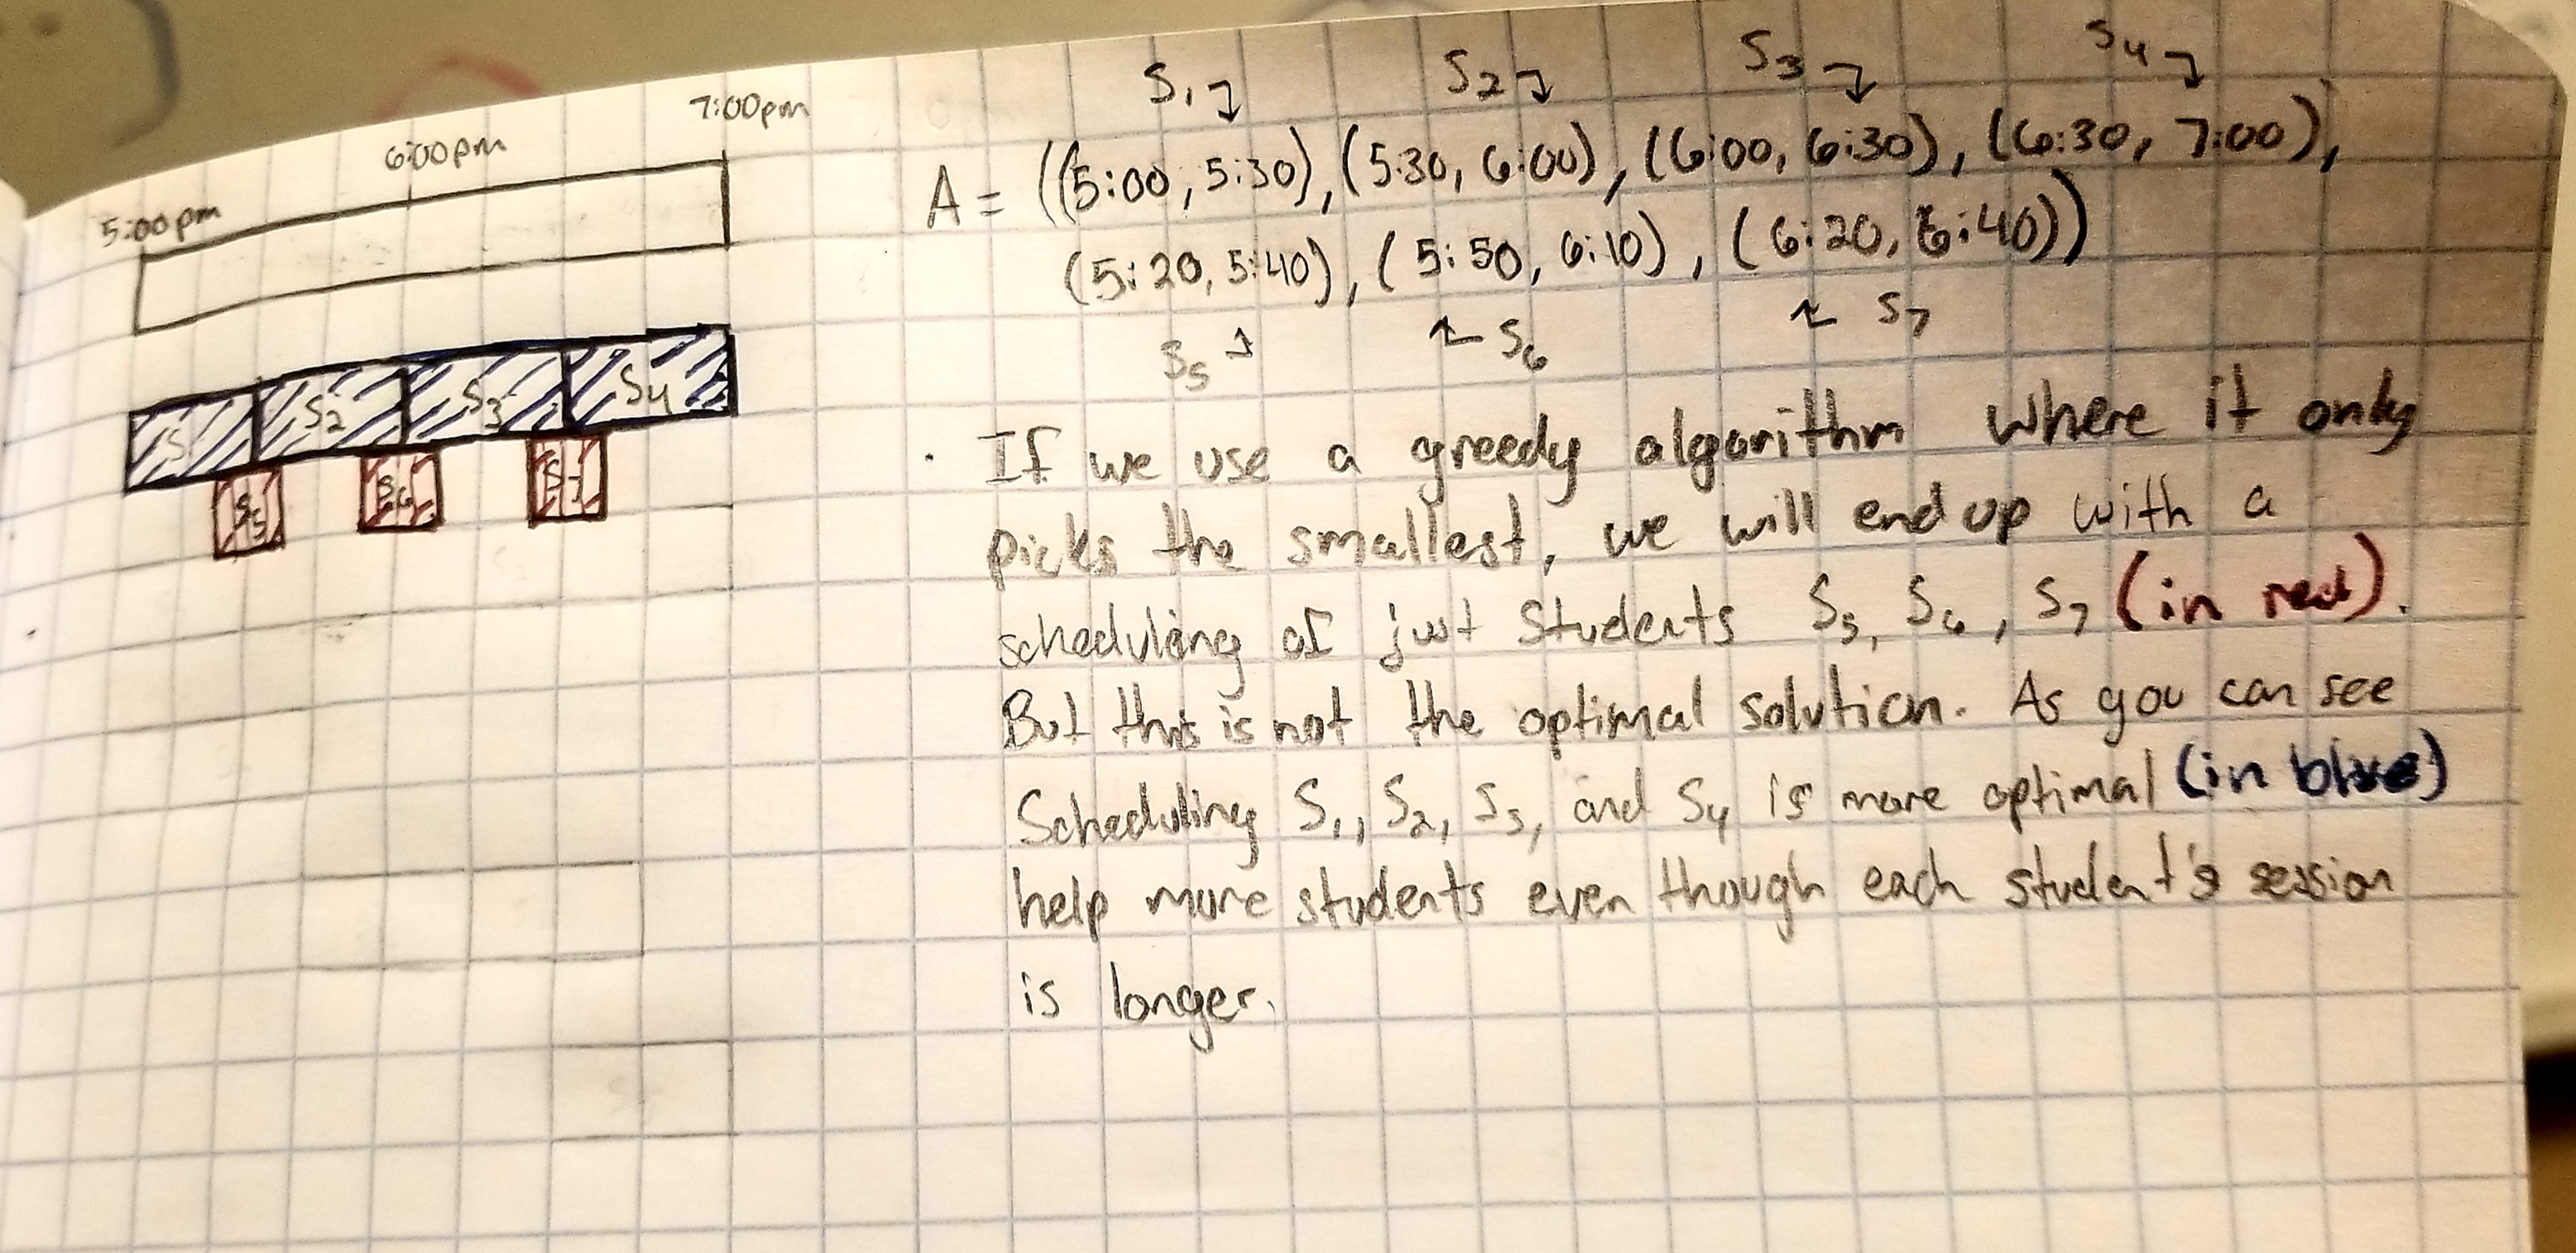
\includegraphics[scale=.15]{1a}
\pagebreak
\item \label{1b} (2 points) Draw an example with at least 5 appointments where a greedy algorithm
    that selects the longest appointment will fail.\\\\
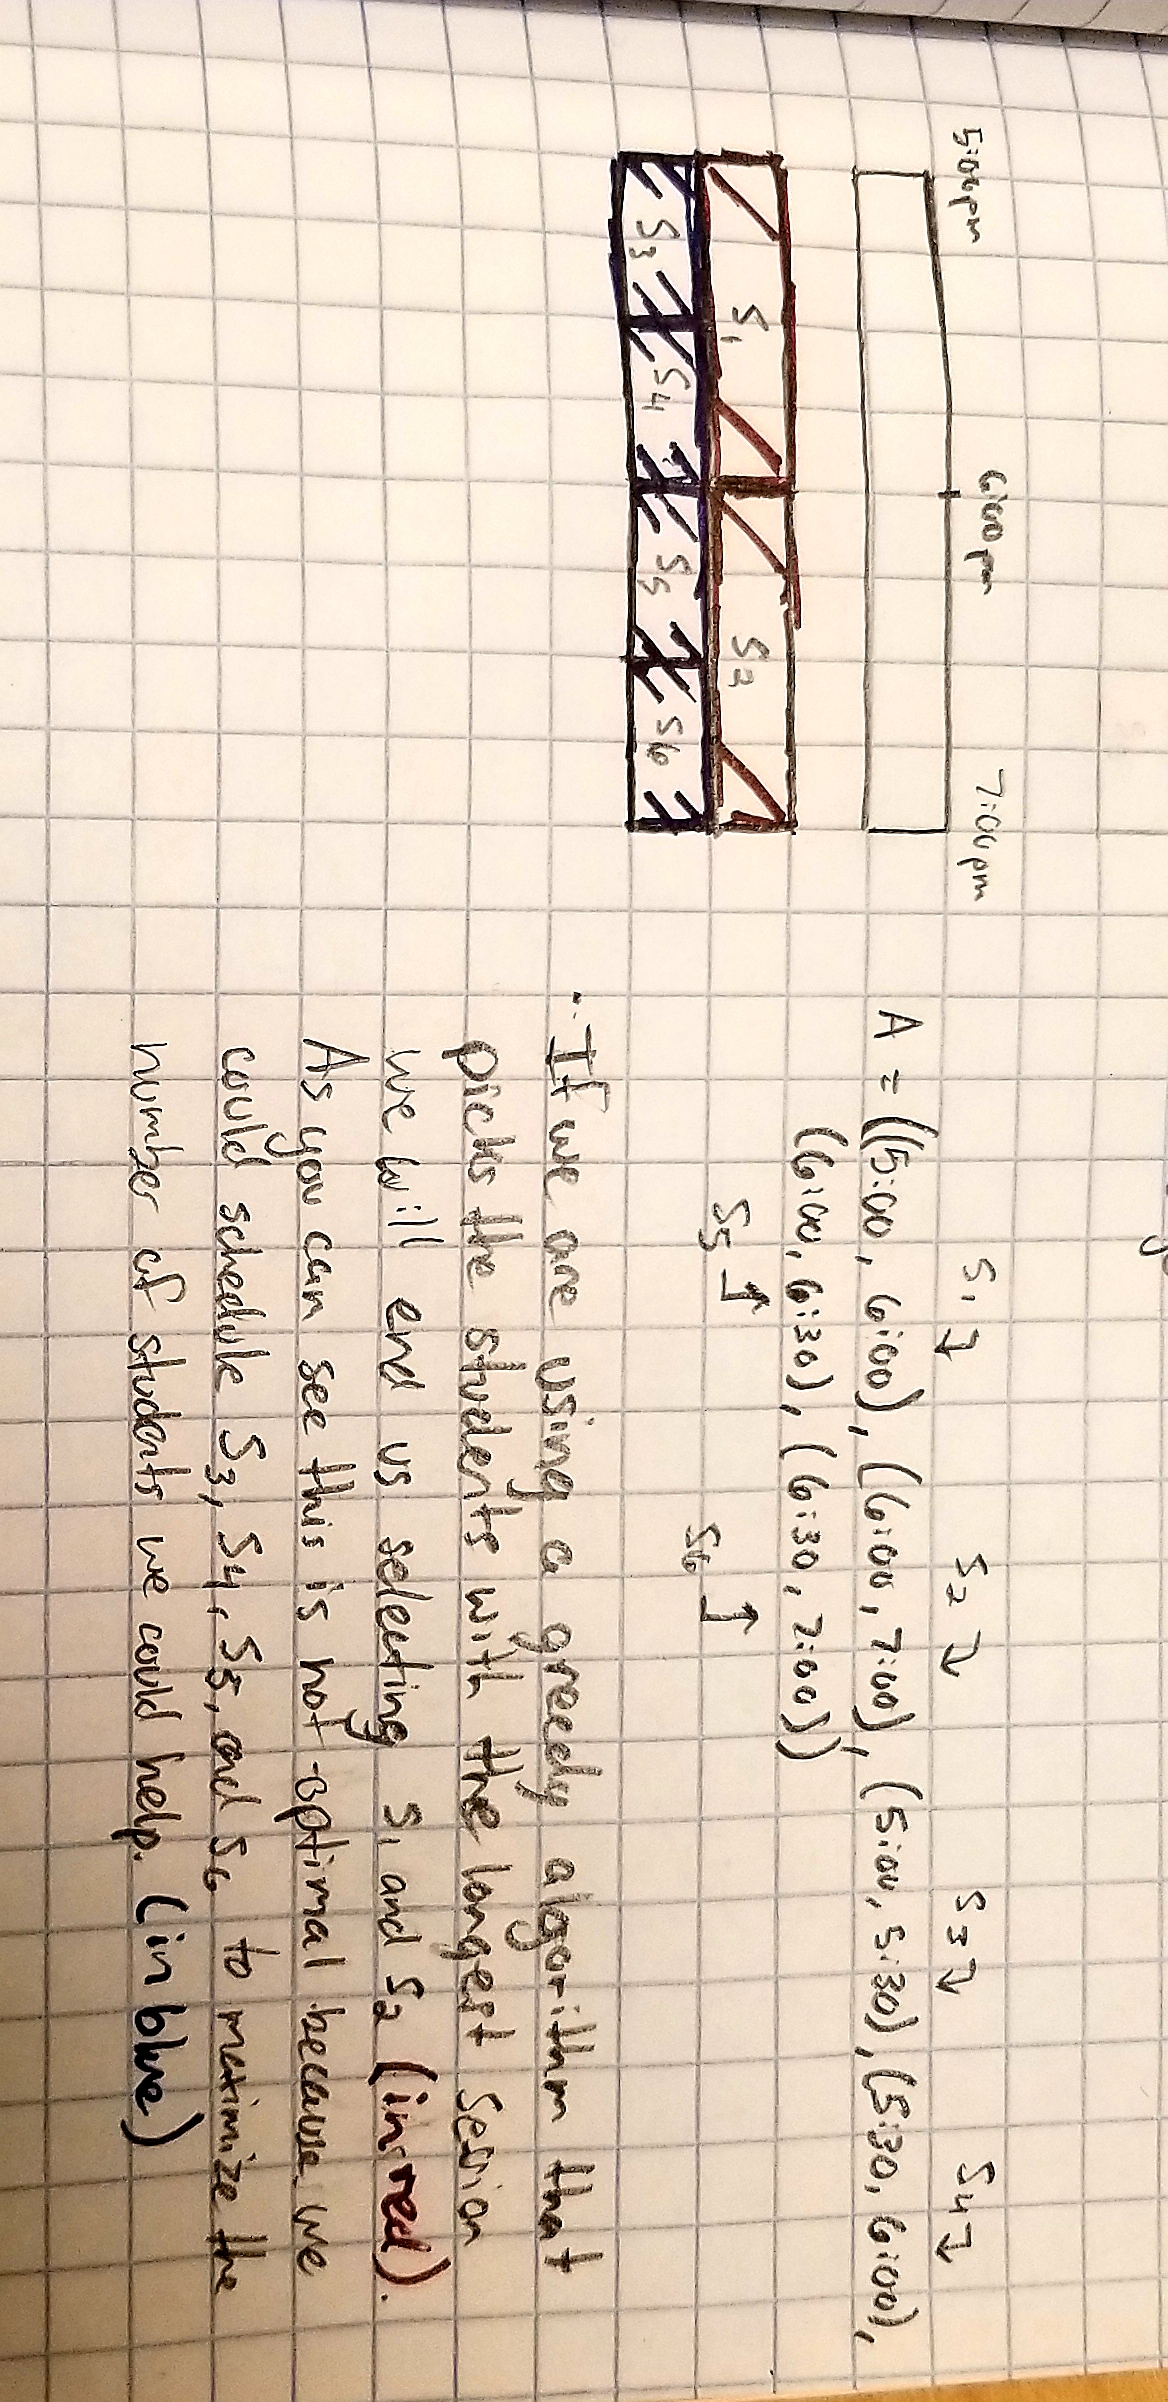
\includegraphics[scale=.17, angle=90]{1b}
\pagebreak
\item \label{1c} (6 points) Describe and prove correctness for a greedy algorithm that is guaranteed
    to choose the subset of appointments that will help the maximum number of
    students that you help.\\\\
    
    \begin{enumerate}
		\item Let GREED = our greedy algorithm, and let U = set of all possible appointments.
		\item Let S = the subset of appointments that maximize the number of students produced by our greedy algorithm 
		\item Let S* be any optional set of appointments, and does not include the greedy choice 
	\end{enumerate}
	{\bf Theorem: }GREED will produce an optimal subset of appointments\\
	{\bf Proof by Contradiction: } \\
	\begin{enumerate}
		\item Since S* is optimal and does not include the greedy choice, we can modify S* with a greedy choice and show it will not take more time. 
		\item In our case, the greedy choice is defined by taking the smallest end - start times, Ex: A =\{(5:00,5:30),(5:30,6:00),(6:00,6:30),(6:30, 7:00),(5:20,5:40),(5:50,6:10),(6:20,6:40)\}, GREED will produce: \{(5:00,5:30),(5:30,6:00),(6:00,6:30),(6:30, 7:00) \}
		\item {\bf Lemma: } If S is a subset of the appointments that maximize the number of students and S* is an optional subset of appointments then for any appointment x, f(k,S) $\leq$ f(k,S*) where f(k,S) and f(k,S*) is the kth time in the greedy algorithm S and the optimal solution S* respectfully.
		\item If we say k = |S| then f(k,S) $\leq$ f(k,S*). In f(k,S*), there exists an k+1 appointment whose start and end time are after f(k,S*) 
		\item We know that S produces a subset of appointments that maximize the number of students which means S = U but if we assume $|S| \textless |S*|$ then S* includes an extra appointment which contradicts U.
		\item By contradiction, the greedy algorithm is optimal
	\end{enumerate}
	\pagebreak
\end{enumerate}

\item %20 points
While your algorithm is clearly efficient and can probably help the most
students, you begin to receive complaints from students that you didn’t
help (i.e., their appointment was not part of the optimal solution).
One of the students even offers to pay extra, which gives you a great
idea. You will now allow students to make a donation to your favorite
charity to make it more likely that their job will be selected. Let
each appointment in this new set of appointments $A$ be a triple 
 $(start_i, end_i, donation_i)$ of start and end times and donation amounts
where $end_i>start_i$ and $donationu_i>0$. You now need to update your
algorithm to handle these donations along with the requested appointment times.
In this new environment, you are trying to maximize the amount of money
you raise for your charity.
\pagebreak

\begin{enumerate}
    \item \label{2a} (2 points) Give a specific case were your greedy algorithm would fail.\\
\includegraphics[scale=.1, angle = 90]{2a}
\pagebreak
    \item \label{2b} (5 points) Give a recursive algorithm that would solve this new case.\\
Def maxDough(A,B,n)\\
\tab if(length(A) == 0):\\
\tab \tab return (b,n)\\
\tab else if(length(A) == 1 and length(B) == 0):\\
\tab \tab n = n + A[0].dontation\\
\tab \tab return (A,n)\\
\tab tempTime = [0][0][0]\\
\tab maxDonation = 0\\
\tab for($i -\textgreater A$)\\
\tab \tab if($i.dontaion \textgreater maxDonation$):\\
\tab \tab maxDonation = i.donation\\
\tab \tab tempTime = i\\
\tab timeColisions = []\\
\tab for($i -\textgreater A$)\\
\tab \tab if(i[0][1] collides with tempTime[o][1] and i != tempTime)\\
\tab \tab \tab timeColisions.append(i)\\
\tab x = maxDonaiton(timeColisions,[],0)\\
\tab if($x[1] \textgreater tempTime.donation$):\\
\tab \tab A.delete(tempTime)\\
\tab \tab maxDonation(A,B,n)\\
\tab else:\\
\tab \tab B.append(tempTime)\\
\tab \tab A.delete(tempTime)\\
\tab \tab n = n + tempTime.donation\\
\tab \tab maxDonation(A,B,n)\\
\pagebreak
    \item \label{2c} (3 points) Add memoization to this algorithm.\\
Def maxDough(A,B,n,memo)\\
\tab if(length(A) == 0):\\
\tab \tab return (b,n)\\
\tab else if(length(A) == 1 and length(B) == 0):\\
\tab \tab n = n + A[0].dontation\\
\tab \tab return (A,n)\\
\tab tempTime = [0][0][0]\\
\tab maxDonation = 0\\
\tab for($i -\textgreater A$)\\
\tab \tab if($i.dontaion \textgreater maxDonation$):\\
\tab \tab \tab maxDonation = i.donation\\
\tab \tab \tab tempTime = i\\
\tab \tab if(i conflicts with memo[tempTime])
\tab \tab \tab memo[tempTime].append(i)
\tab x = maxDonaiton(memo[tempTime,[],0)\\
\tab if($x[1] \textgreater tempTime.donation$):\\
\tab \tab A.delete(tempTime)\\
\tab \tab maxDonation(A,B,n)\\
\tab else:\\
\tab \tab B.append(tempTime)\\
\tab \tab A.delete(tempTime)\\
\tab \tab n = n + tempTime.donation\\
\tab \tab maxDonation(A,B,n)\\
\pagebreak
    \item \label{2d} (10 points) Give a bottom-up dynamic programming algorithm.\\\\
Look at 2c, The memoization makes the algorithm bottom up. 
\pagebreak
\end{enumerate}

\item (30 pts) 
The cashier's (greedy) algorithm for making change doesn't handle arbitrary
denominations optimally. In this problem you'll develop a dynamic
programming solution which does, but with a slight twist. Suppose we
have at our disposal an arbitrary number of \emph{cursed} coins of each
denomination $d_1, d_2, \dotsc, d_k$, with $d_1 > d_2 > \dotsc > d_k$,
and we need to provide $n$ cents in change. We will always have
$d_k=1$, so that we are assured we can make change for any value of
$n$. The curse on the coins is that in any one exchange between people,
with the exception of $i=k-1$, if coins of denomination $d_i$ are used,
then coins of denomination $d_{i+1}$ \emph{cannot} be used. Our goal is
to make change using the minimal number of these cursed coins (in a
single exchange, i.e., the curse applies).
\pagebreak
	
\begin{enumerate}
\item \label{3a} (10 points) For $i \in \{1,\dotsc,k\}$, $n \in \mathbb{N}$, and $b \in \{0,1\}$, let
    $C(i,n,b)$ denote the number of cursed coins needed to make $n$ cents in
    change using only the last $i$ denominations $d_{k-i+1}, d_{k-i+2}, \dotsc, d_k$,
    where $d_{k-i+2}$ is allowed to be used if and only if $i \leq 2$ or
    $b=0$. That is, $b$ is a Boolean ``flag'' variable indicating whether
    we are excluding the next denomination $d_{k-i+2}$ or not ($b=1$ means exclude
    it).Write down a recurrence relation for $C$ and prove it is
    correct. Be sure to include the base case.\\\\
    $$T(n) = 2T(n/2) + C $$
    
    // i = amount of denominations in wallet\\
    // n = change you want to make\\
    //b = if the coin has been used before \\
    
    {\bf f(i,n,b)}\{ 
    \tab //base case\\
    \tab if(n == d[k-i+1])\{ return 1 // return coin\} \\
	\tab if(n == 0) \{ return 0\} \\
	\tab if (i \textless= 1) \{ return n \} \\
	\tab if(D[k-1+1] \textless n) \{ \\
	\tab \tab if(b == 0)\{ return min({\bf f(i,n-d[k-i+1],1)}, {\bf f(i-1,n,0))} \} \\
	\tab \tab else \{ return min({\bf f(i,n-d[k-i+1],1)}, {\bf f(i-2,n,0))}\} \\
	\tab \} \\
	\tab else \{ \\
	\tab \tab if(b == 0)\{ return {\bf f(i-1,n,0)}\} \\
	\tab \tab else \{ return {\bf f(i-2,n,0)}\} \\
	\tab \} \\
	
	If you look at the algorithm I use can see that for a worse case we will always fall the function at least twice each iteration, which is how I go a = 2, and the worst case also includes that every other coin can not be used to maximize the amount of coins that we have to use so the number in the array we pass each time is n/2. Then we add on a constant because we always have the same number of simple atomic operations each iteration. Using Master theorem we find that we get a time complexity of  $\theta(nlongn) $
    
\pagebreak
	
\item \label{3b} (10 points) Based on your recurrence relation, describe the order in
    which a dynamic programming table for $C(i,n,b)$ should be filled in.\\
    
    Based on our code our table should be filled in top down. The recurrence relation builds off of its previous values, but it first fills out all the base cases. We also know that a 3 dimensional table is made with dimensions n by k by 2. The 2 is constructed because of the flags placed on the coins if they have been used or not to determine if we implement the curse or not. The first layer will be b = 0 and the second being b = 1. The case where f(1,n,b) = n' will fill the entire row with n itself, which makes sense because if you are only allowed to use the smallest denomination, then it will be 1 therefore = n.  From there three conditionals are used to determine which recurrence relation is used to fill the table. These recurrence relations will loop through all of the way until they reach their base case, then will roll back up adding a +1 where necessary. Which recurrence relation that is used is determined if the previous coin has been used, and if the n - denomination  $\geq $ 0.   
    
\pagebreak
	
\item \label{3c} (10 points) Based on your description in part (b), write down pseudocode for a
    dynamic programming solution to this problem, and give a $\Theta$ bound on
    its running time (remember, this requires proving both an upper
    \emph{and} a lower bound).\\\\
    d = []\\
    memo = [][][] // table of size k by n by b\\
    f(i,n,b)\{ 
    \tab //base case\\
    \tab if(memo[d[k-i+1]][n][d]) \{ return memo[d[k-i+1]][n][b]\}\\
    \tab else \{ \\
    \tab \tab if(n == d[k-i+1])\{ return 1 // return + 1 coin used\} \\
    \tab \tab if(n == 0) \{ return 0\} \\
	\tab \tab if (i \textless= 1) \{ return n \} \\
	\tab \tab if(d[k-1+1] \textless n) \{ \\
	\tab \tab \tab if(b == 0)\{ value = min(f(i,n-d[k-i+1],1)+1,f(i-1,n,0)\\
	\tab \tab \tab \tab memo[d[k-i+1]][n][b] = value\\
	\tab \tab \tab \tab return value\} \\
	\tab \tab \tab else \{ value = min(f(i,n-d[k-i+1],1)+1,f(i-2,n,0)\\
	\tab \tab \tab \tab memo[d[k-i+1]][n][b] = value\\
	\tab \tab \tab \tab return value\} \\
	\tab \tab \} \\
	\tab \tab else \{ \\
	\tab \tab \tab if(b == 0)\{ return f(i-1,n,0)\} \\
	\tab \tab \tab else \{ return  f(i-2,n,0)\} \\
	\tab \tab \} \\
	
	The new memoized function will have a time of $\theta$ (2{k}n), no matter if it is the worst or the best case. This is proven in the code and it will always fill the entire array for the worst and best case therefor it is the upper and lower bound.

\pagebreak
\end{enumerate}
	
	

\end{enumerate}


\end{document}


